% La Conso — Cover Design System
% Compile with: xelatex design-system-conso.tex
\documentclass[a4paper,11pt]{article}

\usepackage[margin=2.2cm]{geometry}
\usepackage{fontspec}
\usepackage{xcolor}
\usepackage{tikz}
\usepackage{tcolorbox}
\usepackage{graphicx}
\usepackage{tabularx}
\usepackage{booktabs}
\usepackage{colortbl}
\usepackage{pifont}
\usepackage{enumitem}
\usepackage{titlesec}
\usepackage[hidelinks]{hyperref}
\usepackage{fancyhdr}
\usepackage{parskip}
\usepackage{multicol}

\tcbuselibrary{skins,breakable}
\usetikzlibrary{shadows,shadings}

% ─── Fonts ───
\setmainfont{Avenir Next}[
  UprightFont = * Regular,
  BoldFont = * Bold,
  ItalicFont = * Italic,
  BoldItalicFont = * Bold Italic,
]
\setsansfont{Avenir Next}
\setmonofont{Menlo}
\newcommand{\knewave}{\fontspec{Marker Felt}}

% ─── Colors ───
\definecolor{consoBlue}{HTML}{00B4F0}
\definecolor{consoPink}{HTML}{FF4D6A}
\definecolor{consoYellow}{HTML}{FFDC37}
\definecolor{consoNavy}{HTML}{221C46}
\definecolor{consoCoral}{HTML}{FF7375}
\definecolor{consoGreen}{HTML}{2ECC71}
\definecolor{consoText}{HTML}{221C46}
\definecolor{bleenGreen}{HTML}{00C48C}
\definecolor{pageBg}{HTML}{FAFAF8}
\definecolor{cardBg}{HTML}{FFFFFF}
\definecolor{grayLight}{HTML}{F3F4F6}
\definecolor{grayMid}{HTML}{9CA3AF}
\definecolor{grayDark}{HTML}{4B5563}

\pagecolor{pageBg}

% ─── Table styling ───
\definecolor{tableHeader}{HTML}{F0F0F0}
\definecolor{tableRowAlt}{HTML}{F8F8F6}
\newcommand{\tableheader}{\rowcolor{tableHeader}\bfseries}

% ─── Header/Footer ───
\pagestyle{fancy}
\fancyhf{}
\renewcommand{\headrulewidth}{0pt}
\fancyfoot[L]{\small\color{grayMid}La Conso Design System — Denis Henin · uixbydenis.eu}
\fancyfoot[R]{\small\color{grayMid}\thepage}

% ─── Custom commands ───
\newcommand{\colorswatch}[3]{%
  \begin{tikzpicture}
    \fill[#1, rounded corners=4pt] (0,0) rectangle (1.2,1.2);
    \node[anchor=west, font=\small\bfseries, text=consoText] at (1.45,0.75) {#2};
    \node[anchor=west, font=\footnotesize\ttfamily, text=grayMid] at (1.45,0.35) {#3};
  \end{tikzpicture}%
}

\newcommand{\sectionrule}{%
  \vspace{4pt}%
  \noindent
\begin{tikzpicture}
    \shade[left color=consoBlue, right color=consoPink] (0,0) rectangle (\textwidth, 2.5pt);
  \end{tikzpicture}%
  \vspace{6pt}%
}

% ─── Section title formatting ───
\titleformat{\section}
  {\fontsize{22}{26}\selectfont\bfseries\sffamily\color{consoText}}
  {\thesection.}{0.5em}{}
\titleformat{\subsection}
  {\fontsize{14}{18}\selectfont\bfseries\sffamily\color{grayDark}}
  {\thesubsection}{0.5em}{}

\newcommand{\tagpill}[2]{%
  \tikz[baseline=(tag.base)]{%
    \node[fill=#1, text=white, rounded corners=3pt, inner sep=3pt, font=\tiny\bfseries] (tag) {#2};%
  }%
}

% ─── tcolorbox styles ───
\tcbset{
  card/.style={
    enhanced,
    colback=cardBg,
    colframe=grayLight,
    boxrule=0.4pt,
    arc=6pt,
    left=12pt, right=12pt, top=10pt, bottom=10pt,
    fonttitle=\bfseries\sffamily,
    coltitle=grayDark,
    drop shadow={shadow xshift=0.5pt, shadow yshift=-1.5pt, opacity=0.12},
    breakable,
  },
  highlight card/.style={
    card,
    borderline north={2pt}{0pt}{consoBlue!70!consoPink},
  }
}

% ─── Do/Don't icons ───
\newcommand{\doitem}[1]{\item[\textcolor{bleenGreen}{\ding{51}}] #1}
\newcommand{\dontitem}[1]{\item[\textcolor{consoPink}{\ding{55}}] #1}

\begin{document}

% ═══════════════════════════════════════════
% TITLE PAGE
% ═══════════════════════════════════════════

\thispagestyle{empty}

\begin{tikzpicture}[remember picture, overlay]
  % Background gradient
  \shade[left color=consoBlue, right color=consoPink]
    (current page.north west) rectangle ([yshift=-9cm]current page.north east);
  % Dark bottom
  \fill[consoNavy]
    ([yshift=-9cm]current page.north west) rectangle (current page.south east);
\end{tikzpicture}

\vspace*{0.8cm}

\begin{center}
  % Title — text layer (no PNG available yet in layers/)
  {\knewave\fontsize{64}{64}\selectfont\color{white}La Conso}\\[6pt]
  {\Large\color{white}\bfseries Cover Art — Design System}\\[4pt]
  {\small\color{white!60}Version 2.0 — Avril 2026}\\[2pt]
  {\small\color{white!40}Denis Henin — Graphiste Designer @ bleen}
\end{center}

\vspace{0.4cm}

\begin{center}
  \begin{tikzpicture}
    \node[drop shadow={shadow xshift=1pt, shadow yshift=-2pt, opacity=0.3, fill=black}, inner sep=0pt] {%
      \includegraphics[width=7.5cm]{../covers/cover-1-homo-consumens.png}%
    };
  \end{tikzpicture}
\end{center}

\vfill

\begin{center}
  {\footnotesize\color{white!30}Cover « Homo Consumens » · 3000×3000px}
\end{center}

\newpage

% ═══════════════════════════════════════════
% TABLE OF CONTENTS
% ═══════════════════════════════════════════

\tableofcontents
\newpage

% ═══════════════════════════════════════════
% 1. CONTEXTE
% ═══════════════════════════════════════════

\section{Contexte du podcast}
\sectionrule

\begin{tcolorbox}[card]
\rowcolors{2}{white}{tableRowAlt}
\begin{tabularx}{\textwidth}{@{}lX@{}}
\toprule
\tableheader Élément & Détail \\
\midrule
Nom de travail & La Conso (titre final à définir) \\
Tagline & « Toujours plus. Jamais assez. » \\
Format & Podcast audio, format et durée à définir \\
Producteur & Bleen Consulting (Bruxelles) / Bleen Agency (Paris) \\
Lien & S'inscrit dans la lignée de la Fresque de la Consommation \\
Ton & Pédagogique, accessible, questionnement sans culpabilisation \\
Audience & Francophones sensibles à la consommation responsable \\
Thèmes & Consommation responsable, greenwashing, surconsommation, minimalisme, impacts environnementaux \\
Univers visuel & Flat design, gradient bleu-rose, énergie pop \\
\bottomrule
\end{tabularx}
\end{tcolorbox}

\subsection{Positionnement}

Le podcast s'inscrit dans les activités de Bleen autour de la \textbf{Fresque de la Consommation}. C'est un outil de sensibilisation qui décortique les mécanismes de la consommation — publicité, obsolescence, fast fashion, alimentation, impact environnemental. Le ton est celui d'un \textbf{facilitateur}, pas d'un militant.

L'objectif : donner des clés pour comprendre et consommer autrement. Pas de finger-pointing, mais de la pédagogie engagée.

\subsection{Ce que la marque est}

\begin{itemize}[nosep]
  \item Curieuse, engagée, accessible
  \item Un fil rouge entre nos habitudes quotidiennes et leurs impacts
  \item Pédagogique sans être moralisatrice
  \item Optimiste mais lucide — questionner sans culpabiliser
  \item En lien direct avec la Fresque de la Consommation
\end{itemize}

\subsection{Ce que la marque n'est pas}

\begin{itemize}[nosep]
  \item Militant agressif/culpabilisant
  \item Corporate/froid
  \item Anti-consommation radicale
  \item Un simple catalogue de bonnes pratiques
  \item Élitiste ou moralisateur
\end{itemize}

\newpage

% ═══════════════════════════════════════════
% 2. PALETTE DE COULEURS
% ═══════════════════════════════════════════

\section{Palette de couleurs}
\sectionrule

\subsection{Gradient de la cover}

Le fond utilise un \textbf{dégradé horizontal} (gauche $\rightarrow$ droite), bleu ciel vers rose corail. Frais, pop, moderne — distinct des palettes Vélotaf (rouge-orange) et La Grande Démission (indigo-rouge).

\begin{tcolorbox}[card]
\begin{center}
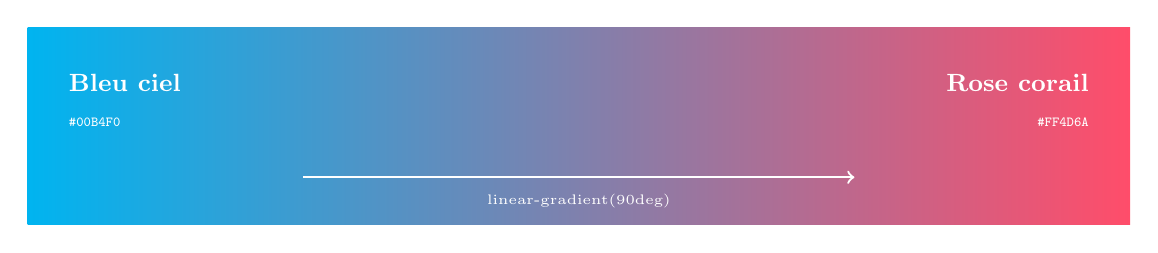
\begin{tikzpicture}
  \shade[left color=consoBlue, right color=consoPink] (0,0) rectangle (14,2.5);
  \node[font=\small\bfseries, text=white, anchor=west] at (0.4, 1.8) {Bleu ciel};
  \node[font=\tiny\ttfamily, text=white, anchor=west] at (0.4, 1.3) {\#00B4F0};
  \node[font=\small\bfseries, text=white, anchor=east] at (13.6, 1.8) {Rose corail};
  \node[font=\tiny\ttfamily, text=white, anchor=east] at (13.6, 1.3) {\#FF4D6A};
  \draw[white, thick, ->] (3.5, 0.6) -- (10.5, 0.6);
  \node[font=\tiny, text=white] at (7, 0.3) {linear-gradient(90deg)};
\end{tikzpicture}
\end{center}
\end{tcolorbox}

\begin{verbatim}
CSS: background: linear-gradient(90deg, #00B4F0, #FF4D6A);
\end{verbatim}

\subsection{Couleurs principales}

\noindent
\colorswatch{consoBlue}{Bleu ciel}{\#00B4F0}\hspace{18pt}%
\colorswatch{consoPink}{Rose corail}{\#FF4D6A}\hspace{18pt}%
\colorswatch{consoYellow}{Jaune solaire}{\#FFDC37}

\vspace{6pt}\noindent
\colorswatch{consoNavy}{Navy profond}{\#221C46}\hspace{18pt}%
\colorswatch{consoCoral}{Corail}{\#FF7375}\hspace{18pt}%
\colorswatch{white}{Blanc}{\#FFFFFF}

\subsection{Rôles des couleurs}

\begin{tcolorbox}[card]
\rowcolors{2}{white}{tableRowAlt}
\begin{tabularx}{\textwidth}{@{}llX@{}}
\toprule
\tableheader Couleur & Hex & Usage \\
\midrule
Bleu ciel & \texttt{\#00B4F0} & Fond gauche du gradient, fraîcheur, questionnement \\
Rose corail & \texttt{\#FF4D6A} & Fond droite du gradient, énergie, urgence douce \\
Jaune solaire & \texttt{\#FFDC37} & Accents, titres sur fond sombre, highlighter \\
Navy profond & \texttt{\#221C46} & Fond alternatif sombre, texte principal, header \\
Corail & \texttt{\#FF7375} & Accent secondaire chaud, variante du rose \\
Blanc & \texttt{\#FFFFFF} & Texte sur gradient, clarté \\
\bottomrule
\end{tabularx}
\end{tcolorbox}

\subsection{Contraste et lisibilité}

\begin{tcolorbox}[highlight card, title=Ratio 60-30-10]
\begin{itemize}[nosep]
  \item \textbf{60\%} — Gradient bleu-rose (fond dominant)
  \item \textbf{30\%} — Blanc pour la typographie et l'air
  \item \textbf{10\%} — Accents (jaune solaire, navy, ou ombres)
\end{itemize}
\end{tcolorbox}

\begin{tcolorbox}[card, title=Interdits, colframe=consoPink!30]
\begin{itemize}[nosep]
  \item Pas de gris moyen (\#888, \#999) — la palette est franche
  \item Pas de pastels — saturation $>$ 30\%
  \item Pas de noir pur (\#000000) — utiliser \texttt{\#221C46}
  \item Pas de vert saturé — éviter le cliché « écolo green »
  \item Pas de violet saturé — LGD utilise déjà du lavande (\texttt{\#9B8EC4}), un violet fort créerait une confusion
\end{itemize}
\end{tcolorbox}

\newpage

% ═══════════════════════════════════════════
% 3. TYPOGRAPHIE
% ═══════════════════════════════════════════

\section{Typographie}
\sectionrule

\subsection{Hiérarchie typographique}

\begin{tcolorbox}[card]
\rowcolors{2}{white}{tableRowAlt}
\begin{tabularx}{\textwidth}{@{}llXl@{}}
\toprule
\tableheader Usage & Police & Justification & Taille \\
\midrule
Logo / Titre & Knewave & Cohérence famille Bleen, énergie brush & variable \\
Sous-titres manuscrits & Caveat (600--700) & Touche personnelle, « fait main » & variable \\
Sous-titres / labels & Plus Jakarta Sans Bold & Lisibilité, modernité & 24--32pt \\
Corps & Plus Jakarta Sans Regular & Neutralité, confort & 14--18pt \\
\bottomrule
\end{tabularx}
\end{tcolorbox}

\subsection{Aperçu du titre sur la cover}

\begin{tcolorbox}[card]
\begin{center}
\includegraphics[width=0.75\linewidth]{../covers/cover-1-homo-consumens.png}
\end{center}

\vspace{6pt}

\rowcolors{2}{white}{tableRowAlt}
\begin{tabularx}{\textwidth}{@{}lX@{}}
\toprule
\textbf{Propriété} & \textbf{Valeur} \\
\midrule
Police titre & Knewave (Google Fonts) \\
Style & Cursive / brush, majuscules \\
Couleur titre & Blanc pur + jaune \texttt{\#FFDC37} pour « Consumens » \\
Stroke & Contour noir semi-transparent (2px dans le card, $\sim$20px à 3000px) \\
Ombre & Text-shadow noir multi-directionnel + glow \\
Paint-order & \texttt{stroke fill} — le contour est peint sous le remplissage \\
\bottomrule
\end{tabularx}
\end{tcolorbox}

\subsection{Traitement du texte sur la cover}

Mêmes principes que Vélotaf et La Grande Démission :

\begin{enumerate}[nosep]
  \item \textbf{Remplissage} : blanc pur \texttt{\#FFFFFF} (titre principal) ou jaune \texttt{\#FFDC37} (accent)
  \item \textbf{Contour (stroke)} : noir semi-transparent, épaisseur adaptée à la résolution
  \item \textbf{Paint-order} : \texttt{stroke fill} — le contour est peint sous le remplissage
  \item \textbf{Ombres} : text-shadow multi-directionnel pour lisibilité sur le gradient
  \item \textbf{Tagline} : police Caveat (handwritten), blanc à 90\% d'opacité
\end{enumerate}

\newpage

% ═══════════════════════════════════════════
% 4. ILLUSTRATION
% ═══════════════════════════════════════════

\section{Illustration}
\sectionrule

\subsection{Style}

\begin{tcolorbox}[card]
\rowcolors{2}{white}{tableRowAlt}
\begin{tabularx}{\textwidth}{@{}lX@{}}
\toprule
\tableheader Propriété & Description \\
\midrule
Type & Illustration vectorielle flat design (cohérence Bleen) \\
Rendu & Semi-réaliste, stylisé (pas cartoon, pas photo-réaliste) \\
Traits & Contours nets, pas de ligne noire visible (formes pleines) \\
Ombres & Minimales, par aplats de couleur plus sombre \\
Fond & Blanc / transparent (détourage, intégration sur gradient) \\
Émotion & Stupéfaction lucide — « c'est absurde et pourtant c'est réel » \\
Perspective & Vue de face ou légère contre-plongée \\
\bottomrule
\end{tabularx}
\end{tcolorbox}

\subsection{Personnage : « Le fil rouge »}

\begin{itemize}[nosep]
  \item Femme tenant un fil rouge qui relie des objets de consommation
  \item Objets reliés : café, sneakers, smartphone, courses
  \item Symbolique : le fil rouge = le podcast qui décortique les liens entre habitudes de conso et impacts
  \item Expression engagée, curieuse, en mouvement
  \item Le personnage occupe $\sim$60\% de la hauteur de la cover
\end{itemize}

\subsection{Fichier source}

\begin{tcolorbox}[card]
\rowcolors{2}{white}{tableRowAlt}
\begin{tabularx}{\textwidth}{@{}lX@{}}
\toprule
\tableheader Fichier & Détail \\
\midrule
\texttt{filRouge.png} & Image source (fond transparent, RGBA) \\
PSD & \texttt{images/filRouge.psd} \\
Dimensions & 1024 × 1024 px \\
Source & Illustration originale, détourée \\
Placement & \texttt{width:95\%; left:-5\%; bottom:-8\%} (à l'échelle 3000px) \\
Filtre & \texttt{drop-shadow(0 4px 12px rgba(0,0,0,0.3))} \\
\bottomrule
\end{tabularx}
\end{tcolorbox}

\subsection{Nettoyage de l'image}

Avant intégration dans la cover :
\begin{itemize}[nosep]
  \item Détourage propre (fond transparent, pas de halo blanc)
  \item Vérification des détails (doigts, objets, proportions)
  \item Cohérence chromatique avec la palette bleu-rose
\end{itemize}

\newpage

% ═══════════════════════════════════════════
% 5. COMPOSITION
% ═══════════════════════════════════════════

\section{Composition \& mise en page}
\sectionrule

\subsection{Structure de la cover (3000×3000px)}

\begin{tcolorbox}[card]
\begin{center}
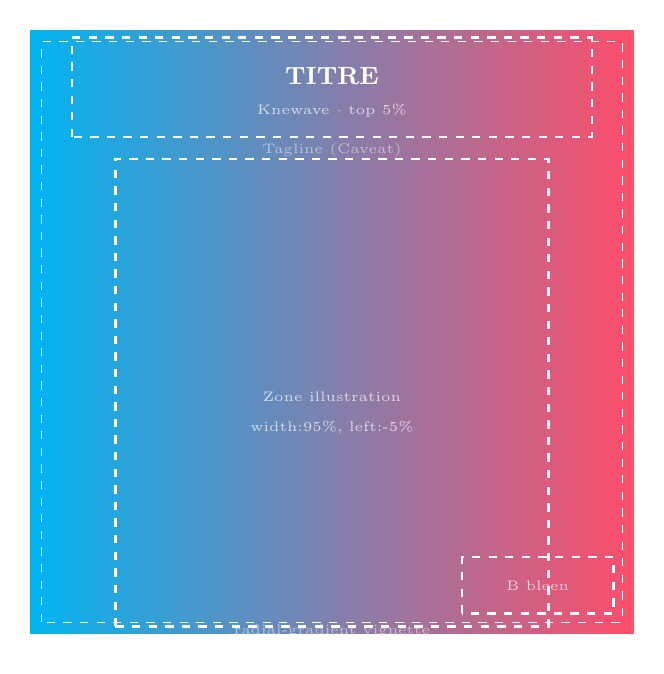
\begin{tikzpicture}[scale=0.55]
  % Cover frame
  \shade[left color=consoBlue, right color=consoPink] (0,0) rectangle (14,14);
  \draw[white, thick] (0,0) rectangle (14,14);

  % Vignette overlay
  \draw[white, dashed, thin] (0.3,0.3) rectangle (13.7,13.7);
  \node[font=\tiny, text=white, opacity=0.5] at (7,0.1) {radial-gradient vignette};

  % Title zone
  \draw[white, dashed, thick] (1,11.5) rectangle (13,13.8);
  \node[font=\small\bfseries, text=white] at (7,12.9) {TITRE};
  \node[font=\tiny, text=white, opacity=0.7] at (7,12.1) {Knewave · top 5\%};

  % Tagline
  \node[font=\tiny, text=white, opacity=0.5] at (7,11.2) {Tagline (Caveat)};

  % Character zone
  \draw[white, dashed, thick] (2,0.2) rectangle (12,11);
  \node[font=\tiny, text=white, opacity=0.7] at (7,5.5) {Zone illustration};
  \node[font=\tiny, text=white, opacity=0.7] at (7,4.8) {width:95\%, left:-5\%};

  % Logo zone
  \draw[white, dashed, thick] (10,0.5) rectangle (13.5,1.8);
  \node[font=\tiny, text=white, opacity=0.7] at (11.75,1.15) {B bleen};
\end{tikzpicture}
\end{center}
\end{tcolorbox}

\subsection{Règles de composition}

\begin{itemize}[nosep]
  \item \textbf{Titre en haut} : toujours au-dessus du personnage, lisible en miniature mobile
  \item \textbf{Personnage centré-gauche} : déborde légèrement à gauche (\texttt{left:-5\%})
  \item \textbf{Fond gradient} : pas de photo, pas de paysage — le gradient suffit
  \item \textbf{Vignette} : radial-gradient sombre en overlay pour encadrer le personnage
  \item \textbf{Espacement généreux} : le design respire, pas d'encombrement
  \item \textbf{Logo} : B bleen regroupés, discret, bas-droite
\end{itemize}

\subsection{Calques d'export}

Chaque cover est exportée en calques séparés (3000×3000px PNG) :

\begin{tcolorbox}[card]
\rowcolors{2}{white}{tableRowAlt}
\begin{tabularx}{\textwidth}{@{}llXl@{}}
\toprule
\tableheader Calque & Fichier & Contenu & Taille \\
\midrule
Background & \texttt{cover-*-bg.png} & Gradient bleu-rose + vignette & $\sim$1.5 MB \\
Personnage & \texttt{cover-*-character.png} & Illustration, fond transparent & $\sim$1.8 MB \\
Texte & \texttt{cover-*-text.png} & Titre + tagline, fond transparent & $\sim$500 KB \\
Logo & \texttt{cover-*-logo.png} & B bleen, fond transparent & $\sim$70 KB \\
\midrule
Composite & \texttt{cover-*.png} & Tous calques fusionnés & $\sim$6 MB \\
\bottomrule
\end{tabularx}
\end{tcolorbox}

\newpage

% ═══════════════════════════════════════════
% 6. LOGO BLEEN
% ═══════════════════════════════════════════

\section{Logo Bleen}
\sectionrule

\subsection{Composition du bloc logo}

Le logo sur la cover utilise un SVG unique avec le viewBox officiel \texttt{0 0 720 280}, garantissant les proportions exactes entre le symbole B et le texte « bleen » :

\begin{tcolorbox}[card]
\rowcolors{2}{white}{tableRowAlt}
\begin{tabularx}{\textwidth}{@{}lX@{}}
\toprule
\tableheader Propriété & Valeur \\
\midrule
SVG & Bloc unique, viewBox \texttt{0 0 720 280} \\
Couleur & \texttt{rgba(255,255,255,0.6)} — blanc à 60\% d'opacité \\
Taille & \texttt{height:25px; width:auto} (preview) / 178px (export 3000px) \\
Position & \texttt{bottom:6\%; right:6\%} \\
Filtre & \texttt{drop-shadow(0 1px 2px rgba(0,0,0,0.2))} \\
\bottomrule
\end{tabularx}
\end{tcolorbox}

\begin{tcolorbox}[card, colframe=consoYellow!50]
\textbf{Note :} Le logo utilise désormais un SVG unifié (identique au SVG du site bleenconsulting.webflow.io) au lieu de deux SVGs séparés (icône + texte). Les ratios sont corrects par construction. Même traitement sur les 3 podcasts (Vélotaf, LGD, La Conso).
\end{tcolorbox}

\subsection{Ratios du logo SVG (source : bleenconsulting.webflow.io)}

Proportions extraites du SVG officiel Bleen (viewBox \texttt{0 0 720 280}) :

\begin{tcolorbox}[card]
\rowcolors{2}{white}{tableRowAlt}
\begin{tabularx}{\textwidth}{@{}lX@{}}
\toprule
\tableheader Mesure & Valeur \\
\midrule
ViewBox global & 720 $\times$ 280 (ratio 18:7 $\approx$ 2.57:1) \\
\midrule
\multicolumn{2}{@{}l}{\textit{Symbole « B »}} \\
Bounding box & x=0$\rightarrow$200, y=0$\rightarrow$280 — soit 200 $\times$ 280 (ratio 5:7) \\
Grand cercle & 200 $\times$ 200 (y=80$\rightarrow$280) \\
Petit cercle & 160 $\times$ 160 (y=0$\rightarrow$160) — ratio petit/grand = 4:5 \\
Chevauchement & 80 unités verticales (y=80$\rightarrow$160) \\
\midrule
\multicolumn{2}{@{}l}{\textit{Texte « bleen »}} \\
Bounding box & x=270$\rightarrow$720, y=70$\rightarrow$210 — soit 450 $\times$ 140 \\
\midrule
\multicolumn{2}{@{}l}{\textit{Rapports clés}} \\
Symbole : Gap : Texte (largeur) & 200 : 70 : 450 ($\approx$ 28\% : 10\% : 62\%) \\
Largeur symbole / largeur texte & 200/450 = 0.444 (le symbole fait 44\% du texte) \\
Hauteur symbole / hauteur texte & 280/140 = 2.0 (le symbole fait 2$\times$ la hauteur du texte) \\
\bottomrule
\end{tabularx}
\end{tcolorbox}

\subsection{Règles}

\begin{itemize}[nosep]
  \item Même traitement que Vélotaf/LGD : icône + texte, bas-droite
  \item Ombre portée pour lisibilité sur le gradient bleu-rose
  \item Zone d'ombre sombre derrière le logo (\texttt{radial-gradient(ellipse at 100\% 100\%, rgba(0,0,0,0.35), transparent 70\%)})
\end{itemize}

\begin{tcolorbox}[card, colframe=consoYellow!50]
\textbf{Note :} Le logo sur les covers utilise \textbf{icône B + logotype « bleen »} ensemble. Les deux éléments restent groupés.
\end{tcolorbox}

\newpage

% ═══════════════════════════════════════════
% 7. EFFETS & OVERLAYS
% ═══════════════════════════════════════════

\section{Effets \& overlays}
\sectionrule

Les covers La Conso utilisent des effets subtils pour donner de la profondeur sans surcharger le visuel.

\begin{tcolorbox}[card]
\rowcolors{2}{white}{tableRowAlt}
\begin{tabularx}{\textwidth}{@{}llX@{}}
\toprule
\tableheader Effet & Intensité & Description \\
\midrule
Vignette & 12--15\% & \texttt{radial-gradient(ellipse, transparent 40\%, rgba(0,0,0,0.12))} \\
Drop-shadow personnage & Léger & \texttt{0 4px 12px rgba(0,0,0,0.3)} \\
Text stroke & 2px (card) & Contour noir semi-transparent autour du titre \\
Text shadow & Multi & Ombre directionnelle + glow diffus \\
Zone logo & 35\% & Radial-gradient sombre, bas-droite, pour lisibilité du logo \\
\bottomrule
\end{tabularx}
\end{tcolorbox}

\subsection{Variantes}

Deux covers retenues, avec des effets légèrement différents :

\begin{tcolorbox}[card]
\rowcolors{2}{white}{tableRowAlt}
\begin{tabularx}{\textwidth}{@{}lXX@{}}
\toprule
\tableheader & Homo Consumens & TROP \\
\midrule
Titre & 2 lignes, blanc + jaune & 1 mot massif, blanc \\
Stroke & 2px \texttt{rgba(0,0,0,0.5)} & 3px \texttt{rgba(0,0,0,0.4)} \\
Shadow & \texttt{0 3px 10px} & \texttt{0 6px 30px} (plus diffus) \\
Tagline & « Toujours plus. Jamais assez. » (Caveat) & Aucune \\
Vignette & Ellipse 90\% & Cercle 30\% $\rightarrow$ 100\% \\
\bottomrule
\end{tabularx}
\end{tcolorbox}

\newpage

% ═══════════════════════════════════════════
% 8. SPECS TECHNIQUES
% ═══════════════════════════════════════════

\section{Spécifications techniques}
\sectionrule

\subsection{Format de la cover}

\begin{tcolorbox}[card]
\rowcolors{2}{white}{tableRowAlt}
\begin{tabularx}{\textwidth}{@{}lX@{}}
\toprule
\tableheader Propriété & Valeur \\
\midrule
Dimensions & 3000 × 3000 px (carré) \\
Résolution & 72 DPI (optimisé écran) \\
Format & PNG 24-bit avec alpha (calques) / PNG opaque (composite) \\
Espace colorimétrique & sRGB \\
Poids composite & $\sim$6 MB \\
Export & Script Python \texttt{covers/generate.py} (Playwright + Pillow) \\
\bottomrule
\end{tabularx}
\end{tcolorbox}

\subsection{CSS de référence}

\begin{tcolorbox}[card, colback=consoNavy, coltitle=white, coltext=white!90]
\begin{verbatim}
/* Gradient de fond */
background: linear-gradient(90deg, #00B4F0, #FF4D6A);

/* Vignette overlay */
background: radial-gradient(ellipse 90% 90% at 50% 50%,
  transparent 40%, rgba(0,0,0,0.12) 100%);

/* Personnage */
width: 95%;
left: -5%;
bottom: -8%;
filter: drop-shadow(0 4px 12px rgba(0,0,0,0.3));

/* Titre (Homo Consumens) */
font-family: 'Knewave', cursive;
color: #ffffff / #ffdc37;
-webkit-text-stroke: 2px rgba(0,0,0,0.5);
paint-order: stroke fill;
text-shadow: 0 3px 10px rgba(0,0,0,0.5);

/* Tagline */
font-family: 'Caveat', cursive;
font-weight: 700;
color: rgba(255,255,255,0.9);

/* Logo B bleen — SVG unifié */
bottom: 6%; right: 6%;
color: rgba(255,255,255,0.6);
height: 25px; width: auto;  /* preview */
filter: drop-shadow(0 1px 2px rgba(0,0,0,0.2));
\end{verbatim}
\end{tcolorbox}

\newpage

% ═══════════════════════════════════════════
% 9. DÉCLINAISONS
% ═══════════════════════════════════════════

\section{Déclinaisons recommandées}
\sectionrule

\subsection{Formats réseaux sociaux}

\begin{tcolorbox}[card]
\rowcolors{2}{white}{tableRowAlt}
\begin{tabularx}{\textwidth}{@{}llX@{}}
\toprule
\tableheader Plateforme & Dimensions & Adaptation \\
\midrule
Instagram post & 1080 × 1080 & Cover art ou variante avec citation \\
Instagram story & 1080 × 1920 & Fond gradient, personnage en bas, titre épisode en haut \\
Bannière Twitter/X & 1500 × 500 & Personnage à gauche, titre + tagline à droite \\
Bannière LinkedIn & 1584 × 396 & Idem Twitter, adapté au format \\
Miniature YouTube & 1280 × 720 & Personnage + titre épisode en gros \\
\bottomrule
\end{tabularx}
\end{tcolorbox}

\subsection{Do's \& Don'ts}

\begin{multicols}{2}
\begin{tcolorbox}[card, title={\color{bleenGreen!80!black}Do's}, colframe=bleenGreen!30, borderline north={2pt}{0pt}{bleenGreen}]
\begin{itemize}[nosep, leftmargin=16pt]
  \doitem{Fond gradient bleu-rose comme élément dominant}
  \doitem{Typo Knewave uniquement pour le titre principal}
  \doitem{Décliner l'illustration dans le même style flat}
  \doitem{Garder le contraste blanc/jaune sur gradient}
  \doitem{Utiliser le jaune solaire pour les accents}
  \doitem{Émotion : stupéfaction lucide — « c'est absurde et pourtant c'est réel »}
\end{itemize}
\end{tcolorbox}

\begin{tcolorbox}[card, title={\color{consoPink}Don'ts}, colframe=consoPink!30, borderline north={2pt}{0pt}{consoPink}]
\begin{itemize}[nosep, leftmargin=16pt]
  \dontitem{Photos en fond}
  \dontitem{Dégradés verticaux ou radiaux comme fond principal}
  \dontitem{Mélanger avec les palettes Vélotaf ou LGD}
  \dontitem{Logo en couleur ou trop visible}
  \dontitem{Surcharger les visuels}
  \dontitem{Noir pur \texttt{\#000000}}
  \dontitem{Ton culpabilisant dans les visuels}
\end{itemize}
\end{tcolorbox}
\end{multicols}

\newpage

% ═══════════════════════════════════════════
% 10. PROCESSUS D'IDÉATION — NAMING
% ═══════════════════════════════════════════

\section{Processus d'idéation — Naming}
\sectionrule

\subsection{Direction client}

Le feedback d'Olivier De Schutter (Bleen) pose trois axes clairs :

\begin{tcolorbox}[highlight card, title=Brief créatif — verbatim Olivier]
\begin{itemize}[nosep]
  \item \textbf{Absurde} — « On peut même aller plus loin dans le côté absurde. » Exemples cités : la ruée du Black Friday, les montagnes de déchets dans le désert.
  \item \textbf{Explicite} — « On peut partir sur un truc plus explicite. » Le nom doit se comprendre sans explication.
  \item \textbf{Conséquences} — Le visuel et le ton doivent montrer les conséquences de la consommation, pas seulement l'acte d'achat.
\end{itemize}
\end{tcolorbox}

\noindent Thèmes confirmés en pré-work : \textbf{greenwashing}, \textbf{surconsommation}, \textbf{lean}, \textbf{minimalisme}.

\subsection{Contraintes de la famille de podcasts}

\begin{tcolorbox}[card]
\rowcolors{2}{white}{tableRowAlt}
\begin{tabularx}{\textwidth}{@{}llX@{}}
\toprule
\tableheader Podcast & Nom & Registre \\
\midrule
La Grande Démission & 3 mots, FR, phénomène social & Sérieux, actuel \\
Vélotaf & 1 mot-valise, FR, néologisme & Familier, dynamique \\
Podcast Conso & ? & Doit s'inscrire dans cette famille \\
\bottomrule
\end{tabularx}
\end{tcolorbox}

\noindent \textbf{Règles implicites :} français (pas d'anglais, pas de latin) · court (1 à 3 mots) · compréhensible sans contexte · distinctif pour une recherche Spotify/Google.

\subsection{Matière première — champ lexical}

Mots et images extraits de la recherche documentaire (47 livres, 11 concepts philo/socio, rapports UNEP/IPCC/FAO).

\begin{multicols}{2}
\begin{tcolorbox}[card, title=Verbes]
déborder · accumuler · jeter · remplacer · remplir · vider · craquer · étouffer · noyer · engloutir · dévorer
\end{tcolorbox}

\begin{tcolorbox}[card, title=Noms]
montagne · trop-plein · spirale · cycle · déchet · surplus · excès · frénésie · boulimie · gavage · crédit
\end{tcolorbox}
\end{multicols}

\begin{tcolorbox}[card, title=Images mentales les plus fortes]
\begin{enumerate}[nosep]
  \item \textbf{La montagne de déchets} — Agbogbloshie, Atacama, décharges textiles
  \item \textbf{La ruée} — Black Friday, portes qui s'ouvrent, la foule sur les promos
  \item \textbf{Le caddie qui déborde} — symbole universel, immédiatement lisible
  \item \textbf{La roue de hamster} — on court, on achète, on court, on achète
  \item \textbf{L'objet qui prend vie} — inspiration Objectus (kashermkens.nl)
\end{enumerate}
\end{tcolorbox}

\subsection{Inspiration externe — Objectus}

Référence apportée par Denis (kashermkens.nl/objectus/) : des objets du quotidien fusionnés avec des formes organiques, créant des créatures hybrides. Surréalisme appliqué aux objets de consommation.

\begin{multicols}{2}
\begin{tcolorbox}[card, title={\color{bleenGreen!80!black}Transférable}, colframe=bleenGreen!30, borderline north={2pt}{0pt}{bleenGreen}]
\begin{itemize}[nosep, leftmargin=12pt]
  \doitem{Objets qui deviennent des entités autonomes}
  \doitem{Uncanny valley appliquée aux objets}
  \doitem{Métaphore : nos objets nous possèdent}
\end{itemize}
\end{tcolorbox}

\begin{tcolorbox}[card, title={\color{consoPink}Non transférable}, colframe=consoPink!30, borderline north={2pt}{0pt}{consoPink}]
\begin{itemize}[nosep, leftmargin=12pt]
  \dontitem{Esthétique sombre, photographique, muséale}
  \dontitem{Noir dominant (la palette Conso est bleu-rose)}
  \dontitem{Rendu réaliste / stop-motion}
\end{itemize}
\end{tcolorbox}
\end{multicols}

\subsection{Inspiration externe — Climax fanzine}

Référence apportée par Olivier. Climax (\texttt{climaxfanzine.fr}) est un fanzine écologique français trimestriel, fondé par Dan Geiselhart et Lauren Boudard. Se définit comme « punk écolo et rigolo ». Slogan : « Le média plus chaud que le climat ». Sans publicité, indépendant, réalisé par des militants.

\begin{tcolorbox}[highlight card, title=ADN Climax — ce qui le définit]
\begin{itemize}[nosep, leftmargin=12pt]
  \item \textbf{Ton sarcastique et décalé} — humour, provocation, tutoiement. Rend l'urgence climatique « cool » et moins anxiogène. « Ton panier est vide... un peu comme les promesses climatiques. »
  \item \textbf{Approche « punk écolo »} — indépendance éditoriale, pas de pub, ton frondeur. Assume une ligne militante sans se prendre au sérieux.
  \item \textbf{Journalisme d'enquête type « polar »} — les articles sont structurés comme des récits d'enquête, pas des tribunes. Du fond derrière l'humour.
  \item \textbf{Rubriques inattendues} — cassent les codes du journalisme environnemental classique. Exemples : « 5 jeux de société qui ont super mal vieilli », « l'écologie va-t-elle ruiner ton couple ? »
  \item \textbf{Esthétique pop} — collage éditorial, photomontages, typo massive qui crie. Chaque numéro a un titre-slogan provocateur (« Les riches vont maigrir », « Ambiance scandale », « Utopie pirate »). Couleurs saturées, jamais vertes.
  \item \textbf{Collaborations illustrateurs} — Maria Medem et autres. L'illustration comme signature identitaire du projet.
  \item \textbf{Anti-anxiogène} — documente une « révolution culturelle écologique ». Le sérieux est dans le fond, la légèreté dans la forme.
\end{itemize}
\end{tcolorbox}

\begin{multicols}{2}
\begin{tcolorbox}[card, title={\color{bleenGreen!80!black}Transférable}, colframe=bleenGreen!30, borderline north={2pt}{0pt}{bleenGreen}]
\begin{itemize}[nosep, leftmargin=12pt]
  \doitem{Collage / montage graphique comme style d'illustration}
  \doitem{Couleurs pop, pas d'esthétique éco-douce}
  \doitem{L'absurde et l'humour comme leviers visuels}
  \doitem{Chaque épisode = identité visuelle propre}
  \doitem{Le titre d'épisode comme accroche « fanzine »}
  \doitem{Énergie punk, authentique, pas corporate}
\end{itemize}
\end{tcolorbox}

\begin{tcolorbox}[card, title={\color{consoPink}Points de divergence}, colframe=consoPink!30, borderline north={2pt}{0pt}{consoPink}]
\begin{itemize}[nosep, leftmargin=12pt]
  \dontitem{Climax n'a pas de charte couleur fixe (nous oui : bleu-rose)}
  \dontitem{Leur typo varie d'un numéro à l'autre (nous : Knewave fixe)}
  \dontitem{Format fanzine papier $\neq$ cover podcast carré}
  \dontitem{Leur densité visuelle (pages pleines) est trop chargée pour une miniature Spotify}
\end{itemize}
\end{tcolorbox}
\end{multicols}

\begin{tcolorbox}[card, colframe=consoYellow!50]
\textbf{Synthèse :} Climax prouve qu'un média écolo peut avoir une identité punk/pop/décalée et que c'est ce décalage qui construit la communauté. Pour le podcast Conso, on garde la palette bleu-rose Bleen et la typo Knewave, mais on emprunte l'esprit \textbf{collage}, le \textbf{ton provocateur}, et le refus de l'esthétique verte cliché. L'illustration de la cover doit montrer les \textbf{conséquences} (déchets, absurde) avec l'énergie Climax, pas avec la douceur d'un magazine développement durable.
\end{tcolorbox}

\newpage

\subsection{Grille d'évaluation}

Chaque nom passe 6 tests. Le critère \textbf{Conséquences} a été ajouté suite au feedback d'Olivier (le nom doit porter l'idée que la conso a des impacts).

\begin{tcolorbox}[card]
\rowcolors{2}{white}{tableRowAlt}
\begin{tabularx}{\textwidth}{@{}lccccccr@{}}
\toprule
\tableheader Nom & Expli. & Absurde & Court & Cherch. & Famille & Conséq. & Total \\
\midrule
\textbf{Planète à Crédit} & \textcolor{bleenGreen}{\ding{51}} & \textcolor{bleenGreen}{\ding{51}} & \textcolor{bleenGreen}{\ding{51}} & \textcolor{bleenGreen}{\ding{51}} & \textcolor{bleenGreen}{\ding{51}} & \textcolor{bleenGreen}{\ding{51}} & \textbf{5.5/6} \\
\textbf{Monde à Vendre} & \textcolor{bleenGreen}{\ding{51}} & \textcolor{bleenGreen}{\ding{51}} & \textcolor{bleenGreen}{\ding{51}} & \textcolor{bleenGreen}{\ding{51}} & \textcolor{bleenGreen}{\ding{51}} & \textcolor{bleenGreen}{\ding{51}} & \textbf{5.5/6} \\
\textbf{Ça Déborde} & \textcolor{bleenGreen}{\ding{51}} & \textcolor{bleenGreen}{\ding{51}} & \textcolor{bleenGreen}{\ding{51}} & \textcolor{bleenGreen}{\ding{51}} & \textcolor{bleenGreen}{\ding{51}} & \textcolor{bleenGreen}{\ding{51}} & \textbf{5.5/6} \\
La Société du Trop & \textcolor{bleenGreen}{\ding{51}} & \textcolor{bleenGreen}{\ding{51}} & \textcolor{bleenGreen}{\ding{51}} & \textcolor{bleenGreen}{\ding{51}} & \textcolor{bleenGreen}{\ding{51}} & $\sim$ & 5/6 \\
Jetable & \textcolor{bleenGreen}{\ding{51}} & \textcolor{bleenGreen}{\ding{51}} & \textcolor{bleenGreen}{\ding{51}} & \textcolor{bleenGreen}{\ding{51}} & \textcolor{bleenGreen}{\ding{51}} & \textcolor{bleenGreen}{\ding{51}} & 5/6 \\
Abondance Zéro & $\sim$ & \textcolor{bleenGreen}{\ding{51}} & \textcolor{bleenGreen}{\ding{51}} & \textcolor{bleenGreen}{\ding{51}} & \textcolor{bleenGreen}{\ding{51}} & \textcolor{bleenGreen}{\ding{51}} & 4.5/6 \\
Gavés & \textcolor{bleenGreen}{\ding{51}} & \textcolor{bleenGreen}{\ding{51}} & \textcolor{bleenGreen}{\ding{51}} & \textcolor{bleenGreen}{\ding{51}} & \textcolor{bleenGreen}{\ding{51}} & $\sim$ & 4.5/6 \\
Assez & \textcolor{bleenGreen}{\ding{51}} & \textcolor{bleenGreen}{\ding{51}} & \textcolor{bleenGreen}{\ding{51}} & \textcolor{consoPink}{\ding{55}} & \textcolor{bleenGreen}{\ding{51}} & $\sim$ & 4/6 \\
TROP & $\sim$ & \textcolor{bleenGreen}{\ding{51}} & \textcolor{bleenGreen}{\ding{51}} & \textcolor{consoPink}{\ding{55}} & \textcolor{bleenGreen}{\ding{51}} & $\sim$ & 3.5/6 \\
Anti-Conso & \textcolor{bleenGreen}{\ding{51}} & $\sim$ & \textcolor{bleenGreen}{\ding{51}} & $\sim$ & \textcolor{bleenGreen}{\ding{51}} & \textcolor{consoPink}{\ding{55}} & 3.5/6 \\
Consommer Moins & \textcolor{bleenGreen}{\ding{51}} & \textcolor{consoPink}{\ding{55}} & \textcolor{bleenGreen}{\ding{51}} & \textcolor{consoPink}{\ding{55}} & \textcolor{bleenGreen}{\ding{51}} & $\sim$ & 3/6 \\
\bottomrule
\end{tabularx}
\end{tcolorbox}

\subsection{Shortlist — Top 3}

\begin{tcolorbox}[highlight card]
\begin{enumerate}[nosep, leftmargin=16pt]

\item \textbf{Planète à Crédit} \tagpill{consoBlue}{TOP 1}\\
On vit à crédit sur les ressources de la Terre. Earth Overshoot Day en trois mots. Porte les conséquences ET l'angle inégalités (qui emprunte~? qui paie~?). Structure identique à « La Grande Démission » (3 mots, phénomène social). Lien direct avec la citation d'O.~De~Schutter.\\
\textit{Tagline :} « On emprunte. On ne rembourse pas. »

\item \textbf{Ça Déborde} \tagpill{consoPink}{TOP 2}\\
Le plus visuel et pop. Le caddie, le placard, la planète — tout déborde. L'absurde qu'Olivier demande, concret et immédiat. Facile à illustrer : des objets qui sortent du cadre.\\
\textit{Tagline :} « Toujours plus. Jamais assez. »

\item \textbf{Monde à Vendre} \tagpill{consoYellow}{TOP 3}\\
Tout est marchandise — la nature, le temps, l'attention. Plus poétique et politique. Fait le lien avec Klein (\textit{No Logo}), Debord (\textit{Spectacle}). Teste si Olivier veut un ton plus engagé.\\
\textit{Tagline :} « Tout a un prix. Mais à quel coût~? »

\end{enumerate}
\end{tcolorbox}

\noindent \textbf{Backup :} La Société du Trop (clin d'œil à Baudrillard) · TROP (semi-validé par Olivier) · Jetable (élégant, un mot).

\subsection{Phrase d'intro — méthode}

Référence : l'intro de \textit{La Grande Démission} suit une structure en 6 temps.

\begin{tcolorbox}[card]
\rowcolors{2}{white}{tableRowAlt}
\begin{tabularx}{\textwidth}{@{}rX@{}}
\toprule
\tableheader \# & Temps \\
\midrule
1 & \textbf{Contexte / déclencheur} — le geste quotidien, banal \\
2 & \textbf{Révélation} — mais derrière ce geste, il y a tout un système \\
3 & \textbf{Accumulation (absurde)} — les chiffres qui claquent \\
4 & \textbf{Question / ouverture} — et si on regardait autrement ? \\
5 & \textbf{Adresse directe} — pour ceux qui se posent des questions \\
6 & \textbf{Mission + signature} — ce qu'on va faire + « Bienvenue sur... » \\
\bottomrule
\end{tabularx}
\end{tcolorbox}

\noindent Le ton est \textbf{oral}, pas écrit. Phrases incomplètes. Du parlé. Une colère douce, pas militante. Et le « Bienvenue » arrive après une respiration.

\subsection{Phrase d'intro — 4 propositions}

\begin{tcolorbox}[highlight card, title=Option 1 — « Le geste anodin » (neutre $\rightarrow$ r\'ev\'elation)]
\textit{Un café ce matin. Un t-shirt en promo. Un colis livré en 24h. Des gestes anodins. Quotidiens. Mais derrière chaque achat, il y a une chaîne. D'extraction. De production. De transport. De déchets. On produit 460 millions de tonnes de plastique par an. On jette un milliard de tonnes de nourriture. Et chaque année, dès le mois de juillet, on a déjà consommé tout ce que la Terre peut nous donner.}\\[4pt]
\textit{Alors pour toutes celles et ceux qui veulent comprendre — pas culpabiliser, comprendre — ce podcast décortique les mécanismes de notre consommation. D'où ça vient, où ça va, et comment on pourrait faire autrement.}\\[4pt]
\textit{(respiration) — Bienvenue sur « [NOM] ».}
\end{tcolorbox}

\begin{tcolorbox}[card, title=Option 2 — « Le crédit » (m\'etaphore $\rightarrow$ syst\`eme)]
\textit{On vit à crédit. Pas celui de la banque. Celui de la planète. Chaque année, on consomme plus que ce que la Terre peut régénérer. Et l'addition, c'est pas nous qui la payons. C'est les océans. Les forêts. Les gens qui fabriquent nos t-shirts à l'autre bout du monde. Consommer, c'est pas juste acheter. C'est aussi les conséquences. La répartition. Qui profite, qui trinque.}\\[4pt]
\textit{Ce podcast, c'est un fil qu'on tire. Celui qui relie nos habitudes quotidiennes à leurs impacts. Sans morale. Sans donner de leçon. Juste en posant les bonnes questions.}\\[4pt]
\textit{(respiration) — Bienvenue sur « [NOM] ».}
\end{tcolorbox}

\begin{tcolorbox}[card, title=Option 3 — « L'absurde » (chiffres $\rightarrow$ questionnement)]
\textit{92 millions de tonnes de vêtements jetés chaque année. 62 millions de tonnes de déchets électroniques. Un milliard de tonnes de nourriture à la poubelle pendant que 783 millions de personnes ont faim. Et nous, on continue. On achète. On jette. On rachète. Comme si c'était normal.}\\[4pt]
\textit{Ce podcast s'arrête un instant. Il regarde ce qu'on met dans nos caddies, ce qu'on jette sans y penser, et ce que tout ça coûte — vraiment. Pas pour faire la morale. Pour comprendre.}\\[4pt]
\textit{(respiration) — Bienvenue sur « [NOM] ».}
\end{tcolorbox}

\begin{tcolorbox}[card, title=Option 4 — « Le fil rouge » (narratif{,} personnel)]
\textit{Tu sais ce truc qu'on ressent parfois en sortant d'un centre commercial ? Ce mélange de satisfaction et de vide. T'as acheté des trucs, mais t'es pas sûr d'en avoir besoin. Et tu te demandes : c'est moi qui ai décidé, ou c'est le système qui a décidé pour moi ?}\\[4pt]
\textit{La publicité, l'obsolescence programmée, le crédit facile, les soldes permanentes... Tout est conçu pour qu'on consomme plus. Et les conséquences — les montagnes de déchets, le plastique dans les océans, les inégalités — on les voit à peine.}\\[4pt]
\textit{Ce podcast tire le fil. Il remonte de nos habitudes à leurs impacts. Avec curiosité, pas avec culpabilité.}\\[4pt]
\textit{(respiration) — Bienvenue sur « [NOM] ».}
\end{tcolorbox}

\subsection{Correspondance intro × nom}

\begin{tcolorbox}[card]
\rowcolors{2}{white}{tableRowAlt}
\begin{tabularx}{\textwidth}{@{}lll@{}}
\toprule
\tableheader Nom & Intro recommandée & Pourquoi \\
\midrule
\textbf{Planète à Crédit} & Option 2 (Le crédit) & La métaphore file naturellement \\
\textbf{Ça Déborde} & Option 3 (L'absurde) & Les chiffres qui s'accumulent = ça déborde \\
\textbf{Monde à Vendre} & Option 1 (Le geste anodin) & La chaîne derrière l'achat \\
\textit{Tout nom} & Option 4 (Le fil rouge) & Universelle, marche avec n'importe quel titre \\
\bottomrule
\end{tabularx}
\end{tcolorbox}

\newpage

% ═══════════════════════════════════════════
% 11. MINDMAP — VUE D'ENSEMBLE
% ═══════════════════════════════════════════

\section{Mindmap — Vue d'ensemble}
\sectionrule

\vspace{6pt}

\begin{center}
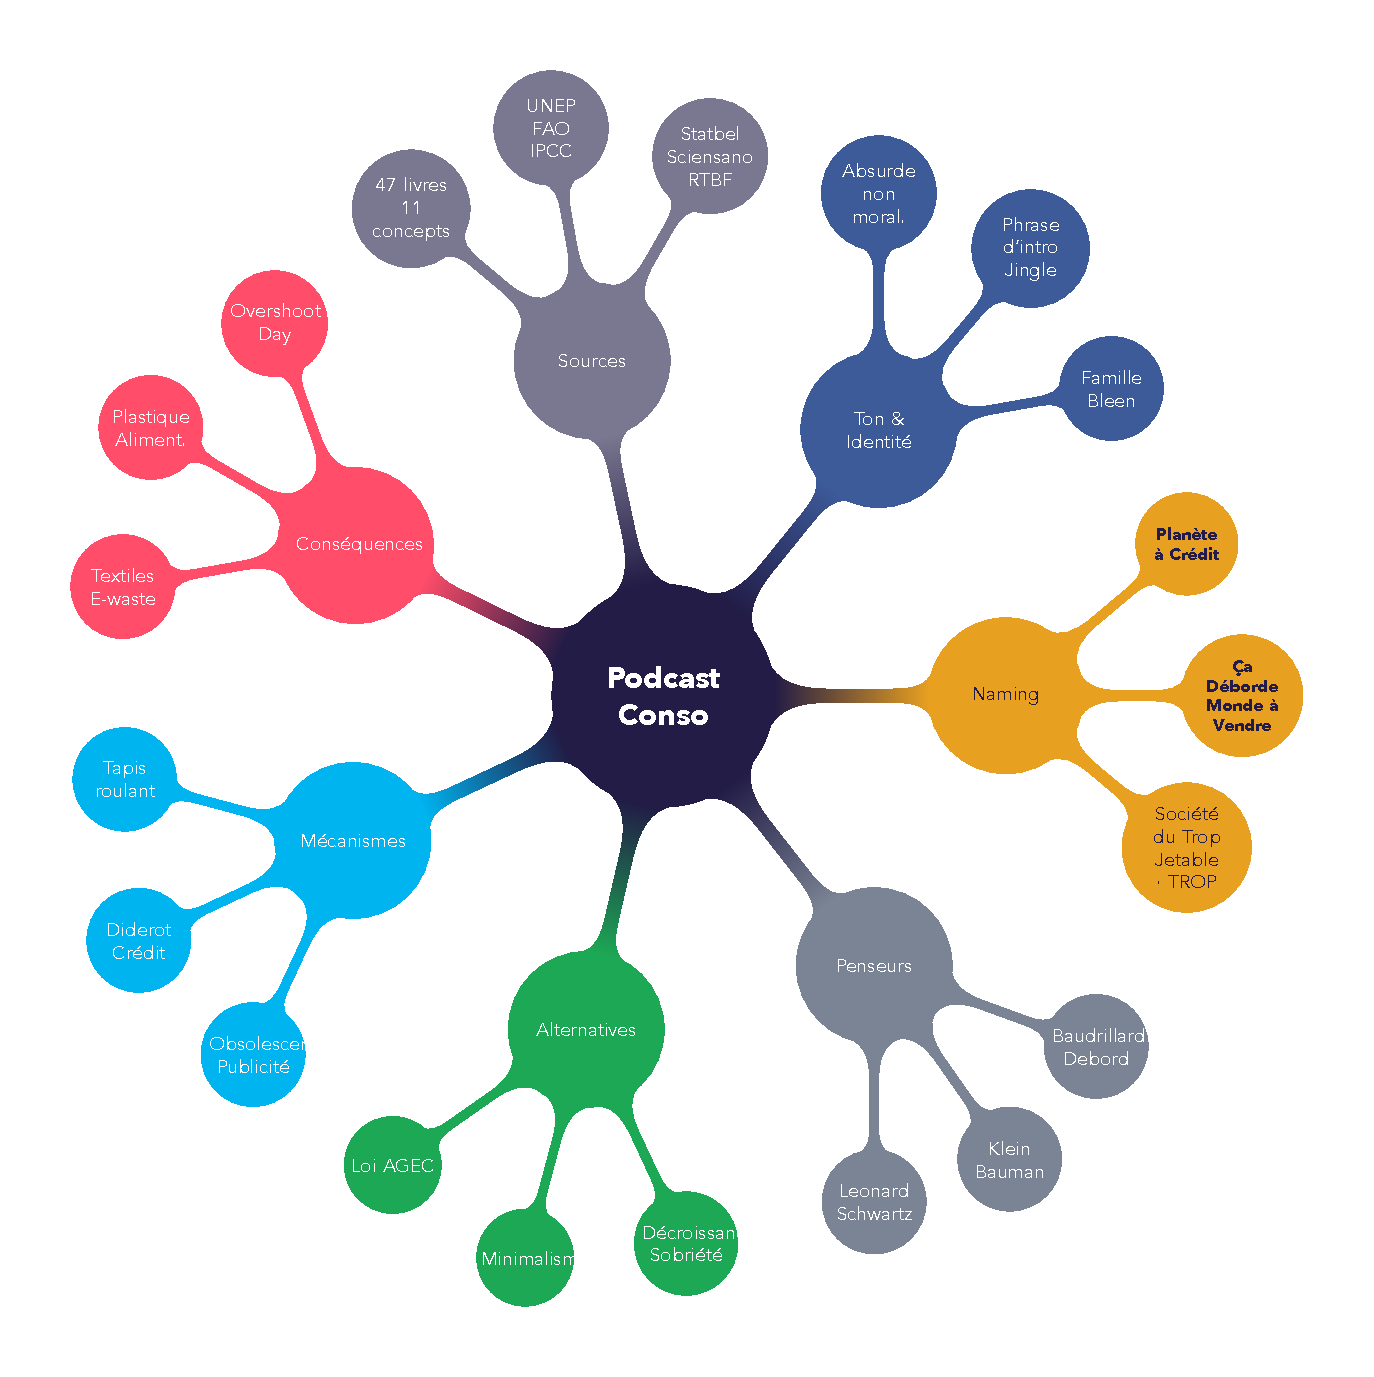
\includegraphics[width=\textwidth]{02-mindmap-ideation.pdf}
\end{center}

\vspace{8pt}

\begin{tcolorbox}[card]
\textbf{Légende des branches :}\\[4pt]
\tagpill{consoPink}{Conséquences} Direction visuelle prioritaire (feedback Olivier)\hfill
\tagpill{consoBlue}{Mécanismes} Ce qui pousse à consommer\\[3pt]
\tagpill{consoYellow}{Naming} Pistes de titres (top 3 en gras)\hfill
\tagpill{bleenGreen}{Alternatives} Pistes de solutions\\[3pt]
\tagpill{grayDark}{Penseurs} Références intellectuelles\hfill
\tagpill{consoBlue!60!consoNavy}{Ton} Identité sonore et visuelle
\end{tcolorbox}

\newpage

% ═══════════════════════════════════════════
% 12. RÉFÉRENCES DOCUMENTAIRES
% ═══════════════════════════════════════════

\section{Références documentaires}
\sectionrule

\subsection{Livres fondamentaux}

\begin{tcolorbox}[card]
\rowcolors{2}{white}{tableRowAlt}
\begin{tabularx}{\textwidth}{@{}lXr@{}}
\toprule
\tableheader Auteur & Titre & Année \\
\midrule
Veblen & \textit{The Theory of the Leisure Class} — consommation ostentatoire & 1899 \\
Debord & \textit{La Société du Spectacle} — la marchandise colonise la vie & 1967 \\
Baudrillard & \textit{La Société de consommation} — symboles, pas objets & 1970 \\
Klein & \textit{No Logo} — colonisation de l'espace public & 2000 \\
Schwartz & \textit{The Paradox of Choice} — trop de choix = paralysie & 2004 \\
Leonard & \textit{The Story of Stuff} — cycle de vie des objets & 2010 \\
Kempf & \textit{Comment les riches détruisent la planète} — inégalités/écologie & 2007 \\
Rabhi & \textit{Vers la sobriété heureuse} — plaisir dans la simplicité & 2010 \\
Hickel & \textit{Less is More} — la décroissance comme voie & 2020 \\
Parrique & \textit{Ralentir ou périr} — référence FR décroissance & 2022 \\
Hawken & \textit{Drawdown} — 100 solutions climat classées par impact & 2017 \\
Safran Foer & \textit{Eating Animals} — industrie de la viande & 2009 \\
Masset & \textit{Fin du monde, fin du mois, même combat~?} — justice climatique & 2020 \\
\bottomrule
\end{tabularx}
\end{tcolorbox}

\subsection{Chiffres clés — avec sources}

{\footnotesize
\begin{tcolorbox}[card]
\rowcolors{2}{white}{tableRowAlt}
\begin{tabularx}{\textwidth}{@{}lXl@{}}
\toprule
\tableheader Thème & Chiffre & Source \\
\midrule
Earth Overshoot Day & 24 juillet 2025. 2,9 Terres si tout le monde vivait comme un Français. & \href{https://www.overshootday.org/}{overshootday.org} \\
Gaspillage alimentaire & 1,05 Mdt/an gaspillées. 19\% de la nourriture disponible. 783M ont faim. & \href{https://www.unep.org/resources/publication/food-waste-index-report-2024}{UNEP 2024} \\
Mode / textile & 92 Mt déchets/an. Mode = 10\% émissions CO2 mondiales. & \href{https://www.unep.org/news-and-stories/story/environmental-costs-fast-fashion}{UNEP 2023} \\
Mode / textile (FR) & Décryptage fast fashion. & \href{https://www.amisdelaterre.org/wp-content/uploads/2023/06/decryptage-fast-fashion-vdef.pdf}{Amis de la Terre 2023} \\
E-waste & 62 Mt en 2022 (+82\% depuis 2010). 22\% recyclés. & \href{https://ewastemonitor.info/}{UNEP/UNITAR 2024} \\
Plastique & 460 Mt/an. 78\,000 microplastiques ingérés/pers/an. & \href{https://www.oecd.org/en/topics/plastics.html}{OECD 2025} \\
Black Friday & 74,4 Mds\$ dépensés. 52\% de regrets. & BCG / Adobe Analytics \\
Inégalité & 20\% de la pop. consomme 80\% des ressources. & \href{https://ourworldindata.org/}{Our World in Data} \\
ODD12 & Rapport consommation et production responsables. & \href{https://www.un.org/sustainabledevelopment/fr/wp-content/uploads/sites/4/2020/03/ODD_12_Rapport2019.pdf}{ONU 2019} \\
Climat (IPCC) & La consommation = levier majeur d'atténuation. & \href{https://www.ipcc.ch/report/ar6/syr/}{IPCC AR6 2023} \\
Alimentation (FAO) & 13\% nourriture perdue entre récolte et vente. & \href{https://www.fao.org/food-loss-and-food-waste/en/}{FAO 2023} \\
Plastique (EU) & Faits, effets et nouvelles règles EU. & \href{https://www.europarl.europa.eu/topics/en/article/20181212STO21610/plastic-waste-and-recycling-in-the-eu-facts-and-figures}{Parlement EU} \\
Budget ménages BE & Données consommation des ménages belges 2022. & \href{https://statbel.fgov.be/fr/themes/menages/budget-des-menages}{Statbel} \\
Nutrition BE & Habitudes nutritionnelles, Bruxelles 2018. & Sciensano (Drieskens et al.) \\
Conso responsable & Baromètre consommation responsable 2025. & \href{https://communication-responsable.ademe.fr/barometre-de-la-consommation-responsable-2025-greenflex-et-lademe}{ADEME / GreenFlex} \\
Biodéchets & Projet Life SEABIL. & \href{https://lifeseabil.fr/projet/life-seabil/}{lifeseabil.fr} \\
\bottomrule
\end{tabularx}
\end{tcolorbox}
}

\subsection{Sources belges et européennes}

\begin{tcolorbox}[card]
\rowcolors{2}{white}{tableRowAlt}
\begin{tabularx}{\textwidth}{@{}lX@{}}
\toprule
\tableheader Source & Contenu \\
\midrule
Statbel (BE) & Enquête budget des ménages, Belgique 2022 \\
Sciensano (BE) & Enquête de santé 2018 : habitudes nutritionnelles, Bruxelles \\
SPF Santé publique (BE) & Sécurité chaîne alimentaire et environnement \\
VRT Max & \textit{Irresistible: Why We Can't Stop Eating} — Chris van Tulleken \\
RTBF Auvio & Investigation — podcasts consommation \\
ADEME / GreenFlex & Baromètre consommation responsable 2025 \\
Parlement Européen & \textit{Plastic in the ocean} — règles EU \\
Amis de la Terre & Décryptage fast fashion (juin 2023) \\
ONU & Rapport ODD12 (2019) \\
\bottomrule
\end{tabularx}
\end{tcolorbox}

\newpage

% ═══════════════════════════════════════════
% 13. NOUVELLES PROPOSITIONS DE COVERS
% ═══════════════════════════════════════════

\section{Nouvelles propositions de covers}
\sectionrule

Suite au feedback client et à la génération d'illustrations punk-pop (style Climax fanzine), 5 nouvelles propositions de covers ont été créées. Chacune teste un titre et une palette couleur différents.

\subsection{Illustrations générées}

7 illustrations originales en style éditorial punk-pop, fond transparent, contours épais, couleurs saturées. Stockées dans \texttt{images/used/}.

\begin{tcolorbox}[card]
\rowcolors{2}{white}{tableRowAlt}
\begin{tabularx}{\textwidth}{@{}lX@{}}
\toprule
\tableheader Fichier & Description \\
\midrule
\texttt{fille-globe-dechets.png} & Femme tenant la Terre sous le bras, déchets qui tombent \\
\texttt{fille-porte-globe.png} & Femme portant le globe, penchée sous le poids \\
\texttt{fille-ensevelie-achats.png} & Femme ensevelie sous sacs, colis, bouteilles (vue frontale) \\
\texttt{fille-noyee-objets.png} & Femme noyée dans une mer d'objets (vue plongeante) \\
\texttt{fille-courses-frenetiques.png} & Femme aux bras chargés, en mouvement, objets en équilibre \\
\texttt{fille-entouree-colis.png} & Femme entourée de colis et paquets \\
\texttt{chariot-surconsommation.png} & Homme poussant un caddie surchargé \\
\bottomrule
\end{tabularx}
\end{tcolorbox}

\subsection{Covers proposées}

\begin{tcolorbox}[card]
\rowcolors{2}{white}{tableRowAlt}
\begin{tabularx}{\textwidth}{@{}clllX@{}}
\toprule
\tableheader \# & Titre & Illustration & Couleur titre & Positionnement \\
\midrule
1 & Planète à Crédit & fille-globe-dechets & Blanc pur & Titre aligné droite, 1 mot/ligne. Illus. calée gauche (\texttt{left:-3\%}, 78\%) \\
2 & Planète à Crédit & fille-porte-globe & Blanc pur & Idem cover 1. Illus. calée gauche \\
3 & Ça Déborde & fille-ensevelie-achats & Orange \texttt{\#FF8C42} + blanc & Titre centré. Illus. pleine largeur \\
4 & ASSEZ & fille-noyee-objets & Lilas \texttt{\#C4B5FD} & 1 mot massif. Illus. \texttt{object-fit:cover} 75\% bas \\
5 & Assez & fille-courses-frenetiques & Rouge \texttt{\#FF2D55} & 1 mot. Illus. calée gauche (\texttt{left:-10\%}, 78\%) \\
\bottomrule
\end{tabularx}
\end{tcolorbox}

\subsection{Tests couleurs du titre}

6 couleurs testées sur le gradient bleu-rose, en remplacement du jaune solaire \texttt{\#FFDC37} utilisé jusqu'ici :

\begin{tcolorbox}[card]
\rowcolors{2}{white}{tableRowAlt}
\begin{tabularx}{\textwidth}{@{}llX@{}}
\toprule
\tableheader Couleur & Hex & Rendu sur gradient bleu-rose \\
\midrule
Navy profond & \texttt{\#221C46} & Contraste inversé, effet tampon. Nécessite stroke blanc. \\
Vert menthe & \texttt{\#4ECDC4} & Frais, inattendu. Complément du rose. \\
Orange vif & \texttt{\#FF8C42} & Énergie, chaleur. Complément du bleu. \\
Lilas / lavande & \texttt{\#C4B5FD} & Cohérence famille LGD. Doux, rêveur. \\
Rouge punch & \texttt{\#FF2D55} & Agressif, urgence. « Assez » comme un cri. \\
Crème & \texttt{\#FFF5E1} & Plus doux que blanc pur. Vintage, papier. \\
\bottomrule
\end{tabularx}
\end{tcolorbox}

\subsection{Composition du titre « Planète à Crédit »}

Structure retenue pour les covers 1 et 2 — titre aligné à droite, un mot par ligne :

\begin{tcolorbox}[card, colback=consoNavy, coltext=white!90]
\begin{verbatim}
/* Bloc titre — aligné droite */
position: absolute;
top: 3%; right: 5%;
display: flex;
flex-direction: column;
align-items: flex-end;

/* "Planète" — plus gros */
font-size: clamp(38px, 14vw, 64px);

/* "à" — plus petit */
font-size: clamp(26px, 9vw, 42px);

/* "Crédit" — moyen */
font-size: clamp(34px, 12vw, 56px);
\end{verbatim}
\end{tcolorbox}

\subsection{Décision en attente}

\begin{tcolorbox}[card, colframe=consoYellow!50]
\textbf{À trancher avec Olivier :}
\begin{itemize}[nosep]
  \item Titre définitif : Planète à Crédit, Ça Déborde, ou Assez~?
  \item Couleur du titre : blanc pur, jaune solaire, ou une des 6 variantes~?
  \item Illustration préférée parmi les 7 générées
  \item Tagline (retirée pour l'instant) : la remettre ou pas~?
\end{itemize}
\end{tcolorbox}

\newpage

% ═══════════════════════════════════════════
% 14. ÉVOLUTION V4→V7 — SOBRE & SEXY
% ═══════════════════════════════════════════

\section{Évolution V4→V7 — Sobre \& Sexy}
\sectionrule

\begin{tcolorbox}[highlight card, title=Contexte — Avril 2026]
Suite au feedback d'Olivier (avril 2026), la direction créative a pivoté. Les covers V1→V3 (absurde, bleu-rose, punk-pop) ont été mises de côté au profit d'une direction \textbf{``Sobre \& Sexy''} : donner envie sans déprimer, transition positive, personnage engagé et lumineux.

\textbf{Verbatim Olivier :} ``Make the transition sexy.''
\end{tcolorbox}

\subsection{Nouveau feedback client}

\begin{tcolorbox}[card]
\rowcolors{2}{white}{tableRowAlt}
\begin{tabularx}{\textwidth}{@{}lX@{}}
\toprule
\tableheader Signal & Traduction créative \\
\midrule
``Make the transition sexy'' & L'esthétique doit séduire, pas alarmer. Sortir du registre ``conséquences'' \\
Style cover 11 (crop) & Personnage recadré, gros plan, pas de full-body \\
Contour titre LGD/Vélotaf & Knewave + text-stroke visible, cohérence famille podcasts \\
4 noms préférés & La Vie en Sobre, Juste Assez, Zéro Superflu, La Déconsommation \\
Rose dominant & Rappel Piaf (Édith), énergie française, chaleur \\
\bottomrule
\end{tabularx}
\end{tcolorbox}

\subsection{Nouveaux noms — shortlist}

Les 4 noms retenus suivent une structure ``petit mot + gros mot'' pour le rythme oral et le traitement typographique :

\begin{tcolorbox}[card]
\rowcolors{2}{white}{tableRowAlt}
\begin{tabularx}{\textwidth}{@{}llX@{}}
\toprule
\tableheader Nom & Structure titre & Registre \\
\midrule
La Vie en Sobre & ``La Vie'' (petit) + ``en Sobre'' (gros) & Positif, aspiration, légèreté \\
Juste Assez & ``Juste'' (fantôme) + ``Assez'' (massif) & Équilibre, affirmation calme \\
Zéro Superflu & ``Zéro'' (petit) + ``Superflu'' (gros) & Direct, efficace, nettoyage \\
La Déconsommation & ``La'' (mini) + ``Déconso/mmation'' (split) & Explicite, sérieux, politique \\
\bottomrule
\end{tabularx}
\end{tcolorbox}

\subsection{Nouvelle palette — ``Piaf''}

La palette bleu-rose (sections 2--3) reste documentée comme base historique. La direction V6/V7 introduit une palette centrée sur le rose Piaf :

\vspace{6pt}
\noindent
\colorswatch{consoPink}{Rose Piaf}{\#E8396B}\hspace{18pt}%
\colorswatch{consoNavy}{Navy profond}{\#221C46}\hspace{18pt}%
\colorswatch{consoYellow}{Jaune solaire}{\#FFDC37}

\definecolor{consoPrune}{HTML}{8B2252}
\definecolor{consoPruneNuit}{HTML}{2D1B2E}
\definecolor{consoCreme}{HTML}{FFF5E1}
\definecolor{consoRoseTendre}{HTML}{F7C8D0}
\definecolor{consoPiafClair}{HTML}{FF6B8A}
\definecolor{consoPiafMid}{HTML}{F2A0B0}

\vspace{6pt}
\noindent
\colorswatch{consoPrune}{Bordeaux / Prune}{\#8B2252}\hspace{18pt}%
\colorswatch{consoPruneNuit}{Prune nuit}{\#2D1B2E}\hspace{18pt}%
\colorswatch{consoCreme}{Crème chaud}{\#FFF5E1}

\vspace{6pt}
\noindent
\colorswatch{consoRoseTendre}{Rose tendre}{\#F7C8D0}\hspace{18pt}%
\colorswatch{consoPiafClair}{Piaf clair}{\#FF6B8A}\hspace{18pt}%
\colorswatch{consoPiafMid}{Piaf mid}{\#F2A0B0}

\begin{tcolorbox}[card, title=Gradients V6/V7 les plus utilisés]
\begin{itemize}[nosep]
  \item \textbf{Rose Piaf triple} : \texttt{linear-gradient(135deg, \#E8396B, \#FF6B8A, \#F2A0B0)}
  \item \textbf{Rose vers crème} : \texttt{linear-gradient(180deg, \#FFF5E1 0\%, \#F2A0B0 40\%, \#E8396B 100\%)}
  \item \textbf{Bordeaux vers Piaf} : \texttt{linear-gradient(135deg, \#8B2252, \#E8396B)}
  \item \textbf{Noir vers navy vers Piaf} : \texttt{linear-gradient(160deg, \#0A0A0A, \#221C46 60\%, \#E8396B 100\%)}
  \item \textbf{Piaf vers solaire} : \texttt{linear-gradient(150deg, \#E8396B 0\%, \#FF4D6A 45\%, \#FFDC37 100\%)}
\end{itemize}
\end{tcolorbox}

\subsection{Nouvelles illustrations}

Deux sets d'illustrations ont été générés pour la direction V7 :

\begin{tcolorbox}[card]
\rowcolors{2}{white}{tableRowAlt}
\begin{tabularx}{\textwidth}{@{}llX@{}}
\toprule
\tableheader Set & Fichier & Description \\
\midrule
Illustration A & \texttt{v6-piaf-rose-beret.png} & Femme au béret, tenant une rose, entourée d'objets (livres, tasses, sacs). Format paysage 1254$\times$791. \\
Illustration B & \texttt{v6-piaf-mariniere-titre.png} & Femme en marinière, mains levées/ouvertes, entourée de fleurs et objets. \\
\midrule
\multicolumn{3}{@{}l}{\textit{Illustrations V6 — poses variées}} \\
Libération & \texttt{v6-liberation-bras-ouverts.png} & Bras ouverts, joie, énergie positive \\
Paisible & \texttt{v6-paisible-yeux-fermes.png} & Yeux fermés, sourire serein \\
Joyeuse & \texttt{v6-joyeuse-fond-rose.png} & Rire éclatant, fond rose \\
Hoodie & \texttt{v6-souriante-hoodie-rose.png} & Sourire franc, hoodie rose \\
Wave & \texttt{v6-joyeuse-wave-rose-jaune.png} & Wave joyeuse, objets autour \\
Wave noire & \texttt{v6-joyeuse-wave-fond-noir.png} & Wave joyeuse, fond sombre \\
\bottomrule
\end{tabularx}
\end{tcolorbox}

\begin{tcolorbox}[card, colframe=consoYellow!50]
\textbf{Évolution du style :} Les illustrations V1--V5 (punk-pop, absurde, ``conséquences'') ont laissé place à un personnage \textbf{positif, lumineux, engagé}. Le registre n'est plus la stupéfaction mais l'\textbf{aspiration} — donner envie d'une vie sobre et désirable.
\end{tcolorbox}

\subsection{Traitement typographique V6/V7}

Le titre utilise Knewave avec un \textbf{contour visible} (text-stroke), cohérent avec les covers de La Grande Démission et Vélotaf.

\begin{tcolorbox}[card, colback=consoNavy, coltext=white!90]
\begin{verbatim}
/* V6 — Contour noir (fond rose/clair) */
font-family: 'Knewave', cursive;
color: #FFFFFF / #FFF5E1;
-webkit-text-stroke: 2-3px rgba(0,0,0,0.45);
paint-order: stroke fill;
text-shadow: -2px -2px 0 rgba(0,0,0,0.35),
             2px -2px 0 rgba(0,0,0,0.35),
             -2px 2px 0 rgba(0,0,0,0.35),
             2px 2px 0 rgba(0,0,0,0.35),
             0 4px 12px rgba(0,0,0,0.5);

/* V7 — Contour coloré (plus subtil) */
-webkit-text-stroke: 2-2.5px rgba(255,245,225,0.7);
/* ou */ rgba(232,57,107,0.65);
/* ou */ rgba(255,255,255,0.65);
paint-order: stroke fill;
\end{verbatim}
\end{tcolorbox}

\begin{tcolorbox}[card, title=Split ``petit mot + gros mot'']
\begin{itemize}[nosep]
  \item Le premier mot est plus petit (clamp 22--32px) et en couleur secondaire
  \item Le deuxième mot est massif (clamp 38--68px) et en couleur dominante
  \item Exemples : \textit{``La Vie''} petit $\rightarrow$ \textit{``en Sobre''} gros / \textit{``Juste''} fantôme $\rightarrow$ \textit{``Assez''} lumineux
  \item Le rythme crée une hiérarchie visuelle lisible même en miniature Spotify
\end{itemize}
\end{tcolorbox}

\subsection{Bilan — 66 propositions}

\begin{tcolorbox}[card]
\rowcolors{2}{white}{tableRowAlt}
\begin{tabularx}{\textwidth}{@{}llrX@{}}
\toprule
\tableheader Version & Direction & Nb & Résumé \\
\midrule
V1 & Illustration classique & 1 & Template + dessin DCD centre \\
V2 & Stat percutante & 1 & ``4\% des émissions mondiales'' \\
V3 & Typographique & 1 & Texte seul, grand format \\
V4 & Absurde + collage & 14 & Illustrations punk-pop, gradient bleu-rose \\
V4b & Palettes radicales & 12 & Tests couleurs titre sur gradient \\
V5 & Nouvelles covers & 5 & Planète à Crédit, Ça Déborde, Assez \\
Palette & Palette de départ & 2 & Exploration chromatique \\
V6 & Sobre \& Sexy & 12 & Feedback Olivier, contour titre, personnage positif \\
V7 & Piaf (finalistes) & 6 & 2 illustrations $\times$ 3 noms, direction retenue \\
\midrule
\multicolumn{2}{@{}l}{\textbf{Total}} & \textbf{66} & \\
\bottomrule
\end{tabularx}
\end{tcolorbox}

\subsection{Décision en attente — Avril 2026}

\begin{tcolorbox}[card, colframe=consoYellow!50]
\textbf{À valider avec Olivier :}
\begin{itemize}[nosep]
  \item Cover finale parmi les V7 (illustration A béret ou B marinière ?)
  \item Nom définitif parmi les 4 retenus
  \item Gradient de fond (Piaf triple, bordeaux, noir→Piaf, ou solaire ?)
  \item Consolider le design system une fois la direction verrouillée
\end{itemize}
\end{tcolorbox}

\vfill

\begin{center}

\begin{tikzpicture}
  \shade[left color=consoPink, right color=consoYellow] (0,0) rectangle (\textwidth, 2pt);
\end{tikzpicture}\\[8pt]
{\small\color{grayMid} Document généré le \today\ — Bleen Consulting}
\end{center}

\end{document}
